% This is a Basic Assignment Paper but with like Code and stuff allowed in it, there is also url, hyperlinks from contents included. 

\documentclass[11pt]{article}

% Preamble

\usepackage[margin=1in]{geometry}
\usepackage{amsfonts, amsmath, amssymb}
\usepackage{fancyhdr, float, graphicx}
\usepackage[utf8]{inputenc} % Required for inputting international characters
\usepackage[T1]{fontenc} % Output font encoding for international characters
\usepackage{fouriernc} % Use the New Century Schoolbook font
\usepackage[nottoc, notlot, notlof]{tocbibind}
\usepackage{listings}
\usepackage{xcolor}
\usepackage{blindtext}
\usepackage{hyperref}
\hypersetup{
    colorlinks=true,
    linkcolor=black,
    filecolor=magenta,      
    urlcolor=cyan,
    pdfpagemode=FullScreen,
    }

\definecolor{codegreen}{rgb}{0,0.6,0}
\definecolor{codegray}{rgb}{0.5,0.5,0.5}
\definecolor{codepurple}{rgb}{0.58,0,0.82}
\definecolor{backcolour}{rgb}{0.95,0.95,0.92}

\lstdefinestyle{mystyle}{
    backgroundcolor=\color{backcolour},   
    commentstyle=\color{codegreen},
    keywordstyle=\color{magenta},
    numberstyle=\tiny\color{codegray},
    stringstyle=\color{codepurple},
    basicstyle=\ttfamily\footnotesize,
    breakatwhitespace=false,         
    breaklines=true,                 
    captionpos=b,                    
    keepspaces=true,                 
    numbers=left,                    
    numbersep=5pt,                  
    showspaces=false,                
    showstringspaces=false,
    showtabs=false,                  
    tabsize=2
}

\lstset{style=mystyle}

% Header and Footer
\pagestyle{fancy}
\fancyhead{}
\fancyfoot{}
\fancyhead[L]{\textit{\Large{Advanced Data Structures}}}
%\fancyhead[R]{\textit{something}}
\fancyfoot[C]{\thepage}
\renewcommand{\footrulewidth}{1pt}



% Other Doc Editing
% \parindent 0ex
%\renewcommand{\baselinestretch}{1.5}

\begin{document}

\begin{titlepage}
	\centering

	%---------------------------NAMES-------------------------------

	\huge\textsc{
		MIT World Peace University
	}\\

	\vspace{0.75\baselineskip} % space after Uni Name

	\LARGE{
		Advanced Data Structures\\
		Second Year B. Tech, Semester 4
	}

	\vfill % space after Sub Name

	%--------------------------TITLE-------------------------------

	\rule{\textwidth}{1.6pt}\vspace*{-\baselineskip}\vspace*{2pt}
	\rule{\textwidth}{0.6pt}
	\vspace{0.75\baselineskip} % Whitespace above the title



	\huge{\textsc{
			Addition of Polynomials using Circular Linked Lists
		}} \\



	\vspace{0.5\baselineskip} % Whitespace below the title
	\rule{\textwidth}{0.6pt}\vspace*{-\baselineskip}\vspace*{2.8pt}
	\rule{\textwidth}{1.6pt}

	\vspace{1\baselineskip} % Whitespace after the title block

	%--------------------------SUBTITLE --------------------------	

	\LARGE\textsc{
		Assignment No. 1
	} % Subtitle or further description
	\vfill

	%--------------------------AUTHOR-------------------------------

	Prepared By
	\vspace{0.5\baselineskip} % Whitespace before the editors

	\Large{
		Krishnaraj Thadesar \\
		Cyber Security and Forensics\\
		Batch A1, PA 20
	}


	\vspace{0.5\baselineskip} % Whitespace below the editor list
	\today

\end{titlepage}

\tableofcontents
\thispagestyle{empty}
\clearpage

\setcounter{page}{1}

\section{Objectives}
\begin{enumerate}
	\item To study data structure: Circular Linked List
	\item To Study different operations that could be performed on CLL
	\item To Study Applications of Circular Linked list
\end{enumerate}

\section{Problem Statement}
\textit{Implement polynomial operations using Circular Linked List: Create, Display, Addition and
	Evaluation}
\section{Theory}

\subsection{Brief about Data structure}
Data structure is a storage that is used to store and organize data. It is a way of arranging data on a computer so that it can be accessed and updated efficiently.

Depending on our requirement and project, it is important to choose the right data structure for our project. For example, if we want to store data sequentially in the memory, then you can go for the Array data structure, while if we have something more complex, we may want to opt for graph, or trees.

They are broadly classified into two types:
\begin{enumerate}
	\item Linear Data Structures: Like Arrays, Linked Lists, Stacks, Queues, etc.
	\item Non-Linear Data Structures: Like Trees, Graphs, etc.
\end{enumerate}


\subsection{Circular Linked List}

Circular Linked List is a linked list where all nodes are connected to form a circle. There is no NULL at the end. A circular linked list can be a singly circular linked list or doubly circular linked list.

\begin{figure}[H]
	\centering
	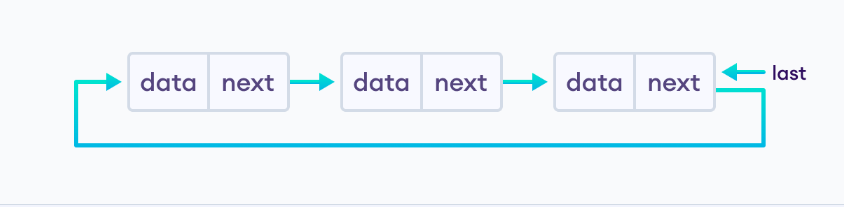
\includegraphics[scale = 0.5]{cll.png}
	\caption{Circular Linked List}
\end{figure}

\subsubsection{Representation using Structures}
\begin{lstlisting}[language=C]
	struct Node {
    int data;
    struct Node * next;
};
\end{lstlisting}

\subsubsection{Advantages of Circular Linked List}

\begin{enumerate}
	\item Any node can be a starting point. We can traverse the whole list by starting from any point. We just need to stop when the first visited node is visited again.
	\item Useful for implementation of queue. Unlike linear data structures, we don’t need to move all elements after a dequeue operation.
	\item Circular lists are useful in applications to repeatedly go around the list. For example, when multiple applications are running in a PC, it is common for the operating system to put the running applications on a list and then to cycle through them, giving each of them a slice of time to execute, and then making them wait while the rest of the applications execute. It is convenient for the operating system to use a circular list so that when it reaches the end of the list it can cycle around to the front of the list.
	\item It is used in multiplayer games to give a chance to each player to play the game.
	\item Multiple running applications can be placed in a circular linked list on an operating system. The os keeps on iterating over these applications.
\end{enumerate}

\subsection{Difference between Singly Linked List, Circular Linked List, and Double Linked List}

\subsubsection{Singly Linked List}

It is the simplest type of linked list. Each node contains two parts: data and pointer to the next node. The last node points to NULL.

\begin{enumerate}
	\item Each node has two parts: data and pointer to the next node.
	\item Each node has only one pointer to the next node.
\end{enumerate}

\begin{figure}[H]
	\begin{small}
		\begin{center}
			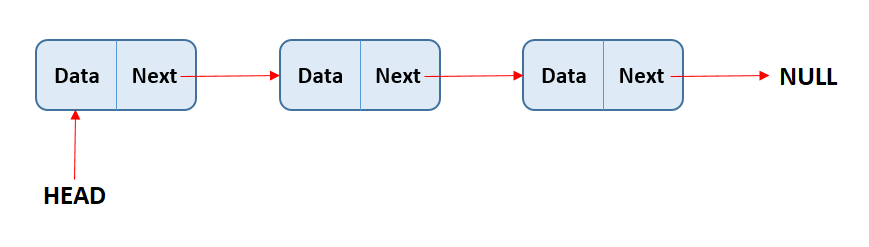
\includegraphics[scale=0.5]{linked-list.png}
		\end{center}
		\caption{}
		\label{fig:}
	\end{small}
\end{figure}


\subsubsection{Circular Linked List}

The Major difference between circular linked list and singly linked list is that the last node of the circular linked list points to the first node of the list.

\begin{figure}[H]
	\begin{small}
		\begin{center}
			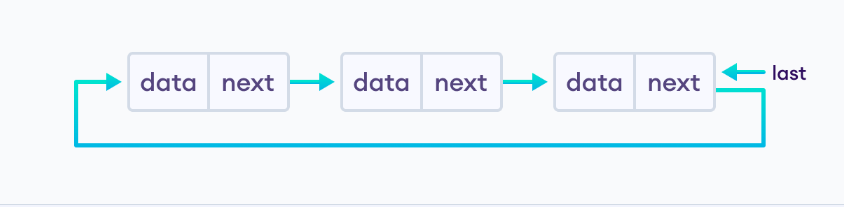
\includegraphics[scale=0.5]{cll.png}
		\end{center}
		\caption{}
		\label{fig:}
	\end{small}
\end{figure}


\subsubsection{Doubly Linked List}

The major difference between doubly linked list and singly linked list is that the doubly linked list has two pointers: one pointer to the next node and another pointer to the previous node.

\begin{figure}[H]
	\begin{small}
		\begin{center}
			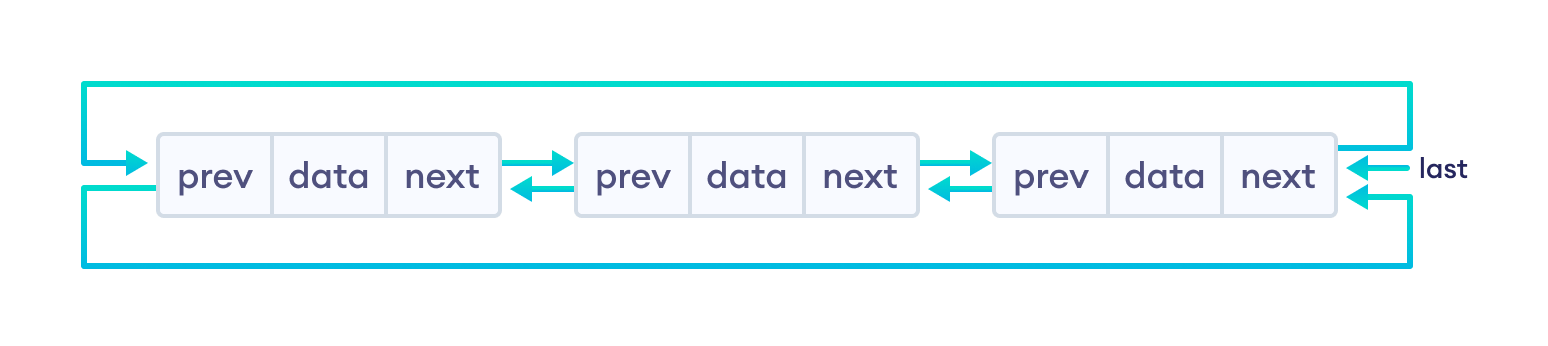
\includegraphics[scale=0.5]{circular-doubly-linked-list.png}
		\end{center}
		\caption{}
		\label{fig:}
	\end{small}
\end{figure}

\subsection{Various operations on CLL}
All the operations that can be performed on any data structure can be performed on a circular linked list. Some of the operations are:
\begin{enumerate}
	\item Insertion
	\item Deletion
	\item Traversal
	\item Search
	\item Sorting
	\item Merging
	\item Reversing
\end{enumerate}

The ADT is a set of operations that can be performed on the data structure. It is given further in the FAQ section. The Pseudo Code for these operations is given in the following sections.


\section{Platform}
\textbf{Operating System}: Arch Linux x86-64 \\
\textbf{IDEs or Text Editors Used}: Visual Studio Code\\
\textbf{Compilers} : g++ and gcc on linux for C++\\

\section{Input}
\begin{enumerate}
	\item The Choice for what to do
	\item The Coefficients and Exponents of the Polynomials
	\item Testcase: Addition of the Following 2 Polynomials
	      \begin{eqnarray}
		      3x^2 + 5x + 9\\
		      4x^6 + 8x
	      \end{eqnarray}
\end{enumerate}
\section{Output}
\begin{enumerate}
	\item The Resultant Polynomial Represented as a Circular Linked List
	\item The Sum of the Given 2 Polynomials.
	\item The Menu for what to do.
	\item Testcase Output:
	      \begin{eqnarray}
		      4x^6 + 8x + 3x^2 + 5x + 9
	      \end{eqnarray}
\end{enumerate}

\section{Test Conditions}
\begin{enumerate}
	\item Input at least five nodes.
	\item Addition of two polynomials with at least 5 terms.
	\item Evaluate polynomial with floating values.
\end{enumerate}

\section{Pseudo Code}
% Write pseudo code for create, display, Addition and evaluation
\subsection{Pseudo Code for Creating a Circular Linked List}

\begin{lstlisting}[language=C]
// Create a circular linked list
void create()
{
	struct node *temp, *ptr;
	int i, n;
	printf("Enter the number of nodes: ");
	scanf("%d", &n);
	for (i = 0; i < n; i++)
	{
		temp = (struct node *)malloc(sizeof(struct node));
		printf("Enter the data: ");
		scanf("%d", &temp->data);
		temp->next = NULL;
		if (head == NULL)
		{
			head = temp;
			ptr = temp;
		}
		else
		{
			ptr->next = temp;
			ptr = temp;
		}
	}
	ptr->next = head;
}

\end{lstlisting}
\subsection{Pseudo Code for Displaying a Circular Linked List}
\begin{lstlisting}[language=C]
// Display a circular linked list

void display(struct Node *head){
	struct Node *ptr = head;
	do{
		printf("%d ", ptr->data);
		ptr = ptr->next;
	}while(ptr != head);
	printf("\n");
}

\end{lstlisting}
\subsection{Pseudo Code for Addition of 2 Polynomials using Circular Linked List}

\begin{lstlisting}[language=C]
struct Node *add_polynomials(struct Node *head1, struct Node *head2)
{
	// Pointers for the result polynomial.
	struct Node *result_head = ASSIGN MEMORY
	result_head->next = result_head;
	struct Node *result_temp = result_head;
	struct Node *result_current;

	// p1 and p2 are the pointers to the first node of the two polynomials.
	struct Node *p1 = head1->next;
	struct Node *p2 = head2->next;

	// In case one of the polynomial exhausts before the other one.
	while (p1 != head1 && p2 != head2)
	{
		// if the exponents are equal, add the coefficients and add the node to the result polynomial.
		if (p1->exp == p2->exp)
		{
			// Copy the data of thesum of the nodes to the result polynomial.
			result_current = ASSIGN MEMORY
			result_current->coeff = p1->coeff + p2->coeff;
			result_current->exp = p1->exp;
			result_current->next = result_head;
			result_temp->next = result_current;

			// Increment the result polynomial pointer, and other polynomial pointers.
			result_temp = result_temp->next;
			p1 = p1->next;
			p2 = p2->next;
		}

		// If the exponent of the first polynomial is greater than the second one, add the node to the result polynomial.
		else if (p1->exp > p2->exp)
		{
			result_current = ASSIGN MEMORY
			result_current->coeff = p1->coeff;
			result_current->exp = p1->exp;
			result_current->next = result_head;
			result_temp->next = result_current;

			// increment the result polynomial pointer, and p1
			result_temp = result_temp->next;
			p1 = p1->next;
		}

		// If the exponent of the second polynomial is greater than the first one, add the node to the result polynomial.
		else if (p2->exp > p1->exp)
		{
			result_current = ASSIGN MEMORY
			result_current->coeff = p2->coeff;
			result_current->exp = p2->exp;
			result_current->next = result_head;
			result_temp->next = result_current;

			// increment the result polynomial pointer, and p2
			result_temp = result_temp->next;
			p2 = p2->next;
		}
	}

	// Case when p2 exhausts before p1.
	if (p1 == head1 && p2 != head2)
	{
		result_temp->next = p2;

		// This loop is to make the last node of the result polynomial point to the head of the result polynomial.
		while (result_temp->next != head2)
		{
			result_temp = result_temp->next;
		}
		result_temp->next = result_head;
	}

	// Case when p1 exhausts before p2.
	else if (p1 != head1 && p2 == head2)
	{
		result_temp->next = p1;
		while (result_temp->next != head1)
		{
			result_temp = result_temp->next;
		}
		result_temp->next = result_head;
	}

	// Case when both p1 and p2 exhaust.
	else if (p1 != head1 && p2 != head2)
	{
		result_temp->next = p1;
		while (result_temp != head1)
		{
			result_temp = result_temp->next;
		}
		result_temp->next = result_head;

		result_temp->next = p2;
		while (result_temp != head2)
		{
			result_temp = result_temp->next;
		}
		result_temp->next = result_head;
	}

	return result_head;
}

\end{lstlisting}
\subsection{Pseudo Code for Evaluation of a Polynomial using a Circular Linked List}

\begin{lstlisting}[language=C]
// evaluate a polynomial using circular linked list
void evaluate(struct Node *head, int x)
{
	struct Node *temp = head->next;
	int result = 0;
	
	// Loop to evaluate the polynomial.
	while (temp != head)
	{
		result += temp->coeff * pow(x, temp->exp);
		temp = temp->next;
	}
	
	printf("The value of the polynomial is %d", result);
}
\end{lstlisting}


\section{Code}

\subsection{Program}
\lstinputlisting[language=C]{../Programs/Assignment_1.c}

\subsection{Input and Output}
\lstinputlisting[]{../Programs/Assignment_1_output.txt}

\section{Conclusion}
Thus, implemented different operations on CLL.
\clearpage

\section{FAQ}

\begin{enumerate}
	\item \textbf{Write an ADT for CLL.}\\

	      \textbf {ADT for CLL is as follows}\\

	      \begin{lstlisting}[language=C]

	// Structure for a node in the circular linked list.
	struct Node
	{
		int data;
		struct Node *next;
	};
	\end{lstlisting}
	      \textbf{Function to create a new node.}
	      \begin{lstlisting}[language=C]

	struct Node *create_node(int data)
	{
		struct Node *new_node = (struct Node *)malloc(sizeof(struct Node));
		new_node->data = data;
		new_node->next = NULL;
		return new_node;
	}
	\end{lstlisting}

	      \textbf{Function to create a circular linked list.}
	      \begin{lstlisting}[language=C]
	
	struct Node *create_circular_linked_list(int data)
	{
		struct Node *head = create_node(data);
		head->next = head;
		return head;
	}

	\end{lstlisting}

	      \textbf{Function to insert a node at the end of the circular linked list.}
	      \begin{lstlisting}[language=C]
	
	struct Node *insert_at_end(struct Node *head, int data)
	{
		struct Node *new_node = create_node(data);
		struct Node *temp = head;
		while (temp->next != head)
		{
			temp = temp->next;
		}
		temp->next = new_node;
		new_node->next = head;
		return head;
	}

		\end{lstlisting}

	      \textbf{Function to insert a node at a given position in the circular linked list.}
	      \begin{lstlisting}[language=C]
	
	struct Node *insert_at_position(struct Node *head, int data, int position)
	{
		struct Node *new_node = create_node(data);
		struct Node *temp = head;
		int i = 1;
		while (i < position - 1)
		{
			temp = temp->next;
			i++;
		}
		new_node->next = temp->next;
		temp->next = new_node;
		return head;
	}
	\end{lstlisting}

	      \textbf{Function to delete a node from the beginning of the circular linked list.}
	      \begin{lstlisting}[language=C]
	
	struct Node *delete_from_beginning(struct Node *head)
	{
		struct Node *temp = head;
		while (temp->next != head)
		{
			temp = temp->next;
		}
		temp->next = head->next;
		free(head);
		head = temp->next;
		return head;
	}
	\end{lstlisting}

	      \textbf{Function to delete a node from a given position in the circular linked list.}
	      \begin{lstlisting}[language=C]
	
	struct Node *delete_from_position(struct Node *head, int position)
	{
		struct Node *temp = head;
		int i = 1;
		while (i < position - 1)
		{
			temp = temp->next;
			i++;
		}
		struct Node *temp2 = temp->next;
		temp->next = temp2->next;
		free(temp2);
		return head;
	}
	\end{lstlisting}

	      \textbf{Function to display the circular linked list.}
	      \begin{lstlisting}[language=C]
	
	void display(struct Node *head)
	{
		struct Node *temp = head;
		while (temp->next != head)
		{
			printf("%d ", temp->data);
			temp = temp->next;
		}
		printf("%d ", temp->data);
		printf(" ");
	}
	\end{lstlisting}

	      \textbf{Function to search for a node in the circular linked list.}
	      \begin{lstlisting}[language=C]
	
	int search(struct Node *head, int data)
	{
		struct Node *temp = head;
		int position = 1;
		while (temp->next != head)
		{
			if (temp->data == data)
			{
				return position;
			}
			temp = temp->next;
			position++;
		}
		if (temp->data == data)
		{
			return position;
		}
		return -1;
	}
	\end{lstlisting}

	      \textbf{Function to sort the circular linked list.}
	      \begin{lstlisting}[language=C]
	
	struct Node *sort(struct Node *head)
	{
		struct Node *temp = head;
		struct Node *temp2 = NULL;
		int temp_data;
		while (temp->next != head)
		{
			temp2 = temp->next;
			while (temp2 != head)
			{
				if (temp->data > temp2->data)
				{
					temp_data = temp->data;
					temp->data = temp2->data;
					temp2->data = temp_data;
				}
				temp2 = temp2->next;
			}
			temp = temp->next;
		}
		return head;
	}

	\end{lstlisting}

	\item \textbf {How to perform multiplication of two polynomials?}\\

	      Multiplication of two polynomials is similar to multiplication of two numbers.
	      \begin{enumerate}
		      \item For each term in the first polynomial, multiply it with each term in the second polynomial.
		      \item While multiplying, add the exponents of the two terms. and Multiply the Coefficients.
	      \end{enumerate}

	\item \textbf { Write polynomial addition algorithm if terms are not sorted.}\\

	      In case the terms are not sorted, we can either sort both the polynomials, and then proceed to add them in the usual way, or we can follow this algorithm

	      \begin{enumerate}
		      \item For each polynomial in the First Polynomial, check for the presence of a term with the same exponent in the other polynomial by looping over it.
		      \item If the term is present, add the coefficients of the two terms, and store the result. Thereby Incrementing the index of the first polynomial.
		      \item If the term is not present, store the term in the result polynomial. Thereby Incrementing the index of the first polynomial.
	      \end{enumerate}

\end{enumerate}


\end{document}